\documentclass{InsightArticle}

\usepackage{tikz}
\usetikzlibrary{arrows,shapes,trees,calc}
\usepackage{graphicx}
%%%%%%%%%%%%%%%%%%%%%%%%%%%%%%%%%%%%%%%%%%%%%%%%%%%%%%%%%%%%%%%%%%
%
%  hyperref should be the last package to be loaded.
%
%%%%%%%%%%%%%%%%%%%%%%%%%%%%%%%%%%%%%%%%%%%%%%%%%%%%%%%%%%%%%%%%%%
\usepackage[dvips,
bookmarks,
bookmarksopen,
backref,
colorlinks,linkcolor={blue},citecolor={blue},urlcolor={blue},
]{hyperref}

\title{N-Dimensional Phase Unwrapping}

%
% NOTE: This is the last number of the "handle" URL that
% The Insight Journal assigns to your paper as part of the
% submission process. Please replace the number "1338" with
% the actual handle number that you get assigned.
%
\newcommand{\IJhandlerIDnumber}{xxxx}

% Increment the release number whenever significant changes are made.
% The author and/or editor can define 'significant' however they like.
\release{0.00}

% At minimum, give your name and an email address.  You can include a
% snail-mail address if you like.
\author{Davis M. Vigneault,$^{1,2,3}$ Wen-Tung Wang, PhD,$^{2}$ Michael Tee,$^{1,2}$ David A. Bluemke, MD, PhD,$^{2}$ and J. Alison Noble, PhD$^{1}$}
\authoraddress{$^{1}$Institute of Biomedical Engineering, Department of Engineering Science, University of Oxford, Oxford, United Kingdom.\\
               $^{2}$Department of Radiology and Imaging Sciences, Clinical Center, National Institutes of Health, Bethesda, MD, United States.\\
               $^{3}$Sackler School of Graduate Biomedical Sciences, Tufts University School of Medicine, Boston, MA, United States.}

\usepackage{amsmath}
\begin{document}

%
% Add hyperlink to the web location and license of the paper.
% The argument of this command is the handler identifier given
% by the Insight Journal to this paper.
%
\IJhandlefooter{\IJhandlerIDnumber}


\ifpdf
\else
   %
   % Commands for including Graphics when using latex
   %
   \DeclareGraphicsExtensions{.eps,.jpg,.gif,.tiff,.bmp,.png}
   \DeclareGraphicsRule{.jpg}{eps}{.jpg.bb}{`convert #1 eps:-}
   \DeclareGraphicsRule{.gif}{eps}{.gif.bb}{`convert #1 eps:-}
   \DeclareGraphicsRule{.tiff}{eps}{.tiff.bb}{`convert #1 eps:-}
   \DeclareGraphicsRule{.bmp}{eps}{.bmp.bb}{`convert #1 eps:-}
   \DeclareGraphicsRule{.png}{eps}{.png.bb}{`convert #1 eps:-}
\fi


\maketitle


\ifhtml
\chapter*{Front Matter\label{front}}
\fi

\begin{abstract}

\noindent

Although phase data can take on any value, it is generally only possible to measure phase as a \emph{principle} value, i.e., wrapped within the range $(-\pi, \pi]$.  Determining the unwrapped phase from its principle value is a topic of considerable interest in magnetic resonance imaging (MRI), as well as many non-medical disciplines.  Despite their importance in image analysis, filters for manipulating phase information have not been incorporated into ITK.  This article introduces the ITKPhase module, containing filters useful for understanding, analyzing, and unwrapping $n$-dimensional phase data, and also serves as a practical introduction to phase unwrapping.

\end{abstract}

\IJhandlenote{\IJhandlerIDnumber}

\tableofcontents
\clearpage
\section{Background}

\subsection{Theory}

Data collected via magnetic resonance (MR) imaging is inherently complex-valued, containing both real and imaginary (or equivalently, phase and magnitude) components (Figure~\ref{fig:Complex_Plane}).  Phase data is useful in a variety of applications, such as harmonic phase (HARP) analysis of tagged MR \cite{Osman1999}, susceptibility weighted imaging (SWI) \cite{Li2011}, and phase contrast angiography/venography .  Although phase at a given pixel can generally take on any value, it is impossible to distinguish between true ($\phi$) and principal ($\hat{\phi}$) phase values separated by an arbitrary multiple $k$ of $2\pi$, such that the measured phase value is `wrapped' within the range $(-\pi, \pi]$.  In theory, true phase may be recovered from principle phase by adding an integer multiple $k$ of $2\pi$, in a process known as `unwrapping' (Equation~\ref{eqn:PrinciplePhase}).

\begin{equation}
\label{eqn:PrinciplePhase}
\phi = \hat{ \phi } + k2\pi
\end{equation}

\begin{figure}[h] % h indicates inline
\center
\begin{tikzpicture}[scale=2.5]
\draw [very thin, lightgray] (0,0) circle [radius=1]; % circle
\draw [<->, black] (-1.2,0) -- (1.2,0); % imaginary
\draw [<->, black] (0,-1.2) -- (0,1.2); % real
\draw [->, thick, gray] (0.7071,0) -- (0.7071,0.7071); % b
\draw [->, thick, gray] (0,0) -- (0.7071, 0); % a
\draw [->, very thick, teal] (0,0) -- (0.7071,0.7071); % R
\node [above right] at (0.2,0) {$\hat{\phi}$};
\node [below] at (0.3535, 0) {$a$};
\node [right] at (0.7071, 0.3535) {$b$};
\node [above left] at (0.3535, 0.3535) {$R$};
\node [right] at (1.2, 0) {Real};
\node [above] at (0, 1.2) {Imaginary};
\end{tikzpicture}
\itkcaption[Complex_Plane]{The Complex Plane.  Here a complex number, $z$, is represented as a point on the complex plane.  $z$ can be represented equivalently in cartesian coordinates as the sum of a real and an imaginary number ($z = a+bi$) or in polar coordinates as a magnitude phase pair ($[R,\phi]$).}
\label{fig:Complex_Plane}
\end{figure}

The reverse operation, by which principle phase is obtained from its true phase, is denoted by the wrapping operator $W{}$ (Equation~\ref{eqn:Wrapping_Operator}), which can be practically implimented with the four-quadrant arctangent function (\code{std::atan2(x,y)}).

\begin{equation}
\label{eqn:Wrapping_Operator}
\hat{\phi} = \arctan( \sin( \phi ), \cos( \phi )) \equiv W \left\{ \phi \right\}
\end{equation}

Itoh \cite{Itoh1982} observed that the locally `corrected' phase gradient (i.e., the phase gradient after appropriate addition of $k2\pi$ such that the difference between adjacent pixels is in the range $(-\pi,\pi]$) may be written in terms of the wrapping operator (Equation~\ref{eqn:Wrapped_Phase_Gradient}).\footnote{$i$ is used in this submission both to refer to the mathematical constant meaning $\sqrt{-1}$, as previously, and, in this context, to pixel index along an arbitrary dimension ($0 < i < M-1$, where M is the number of pixels along that dimension).  The difference in usage should be clear from context.  Note also that the above definition only applies when both $i$ and $i-1$ are completely within the image; otherwise, $\Delta \phi_i \equiv 0$.}

\begin{equation}
\label{eqn:Wrapped_Phase_Gradient}
\Delta \phi_{i} \equiv W \left \{ \hat{\phi_{i}} - \phi_{i-1} \right \}
\end{equation}

A target pixel ($\phi_{i}$) may be `unwrapped' relative to an adjacent reference pixel ($\phi_{i-1}$) such that their difference is in the range $(-\pi, \pi]$.  This operation can be written in terms of the wrapped phase gradient (Equation~\ref{eqn:Binary_Unwrap}).

\begin{equation}
\label{eqn:Binary_Unwrap}
\phi_{i} = \phi_{i-1} + \Delta \phi_{i}
\end{equation}

\subsection{Introduction to the ITKPhase Module}

The presented module provides the unary wrap operator as a functor, \code{itk::Functor::WrapPhaseFunctor} (defined in \code{itkWrapPhaseFunctor.h}).  The following snippet demonstrates the basic use of the class.\footnote{The constant \code{vnl\_math::pi} is defined in the \code{vnl/vnl\_math.h} header file. \code{std::cout} and \code{std::endl} are defined in the \code{<iostream>} header file.}

\small
\begin{verbatim}
  itk::Functor::WrapPhaseFunctor< double > wrapFunc;

  std::cout << wrapFunc( 3 ) << std::endl; // 3
  std::cout << wrapFunc( 0 ) << std::endl; // 0
  std::cout << wrapFunc( -3 ) << std::endl; // -3
  std::cout << wrapFunc( 1 + vnl_math::pi ) << std::endl; // -2.14159
  std::cout << wrapFunc( -vnl_math::pi - 1 ) << std::endl; // 2.14159
\end{verbatim}
\normalsize

\code{itk::PhaseImageToImageFilter} (defined in \code{itkPhaseImageToImageFilter.h}) inherits from \doxygen{ImageToImageFilter} and serves as the base class for most classes in this module.

This class provides two methods, \code{Wrap(pixel)} and \code{Unwrap(target,relativeToReference)}.  The first takes one argument and provides an interface to \code{WrapPhaseFunctor} (see Equation~\ref{eqn:Wrapping_Operator}).  The second makes use of the first to unwrap one pixel relative to another (see Equation~\ref{eqn:Binary_Unwrap}).

\begin{figure}[h]
\center


\includegraphics[width=0.24\textwidth]{images/2/00a_ramp_wrapped.png}

\includegraphics[width=0.24\textwidth]{images/2/00b_ramp_unwrapped.png}
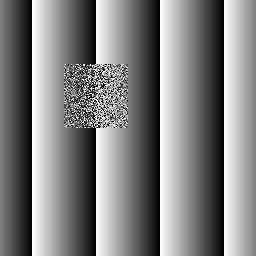
\includegraphics[width=0.24\textwidth]{images/2/00c_noise_wrapped.png}

\includegraphics[width=0.24\textwidth]{images/2/00d_noise_unwrapped.png}

\itkcaption[Simulated_Phase_Examples]{Simulated phase images, created by the \code{itk::PhaseExamplesImageSource} class.  Wrapped phase ramp (far left); wrapped phase ramp with noise patch (center left); unwrapped phase ramp (center right); unwrapped phase ramp with noise patch (far right).}
\label{fig:Simulated_Phase_Examples}
\end{figure}

For convenience, the ITKPhase module also includes \code{itk::PhaseExamplesImageSource} (defined in \code{itkPhaseExamplesImageSource.h}), which provides simple simulated phase examples for demonstrating the functionality of the module's classes.

By default, the class outputs a simple, wrapped phase ramp (Figure~\ref{fig:Simulated_Phase_Examples}, far left).\footnote{For visualization purposes, all images have been rescaled prior to writing to png.}

\small
\begin{verbatim}
  typedef itk::PhaseExamplesImageSource< WorkImageType > ExampleType;
  ExampleType::Pointer phase = ExampleType::New();
  phase->Update();
\end{verbatim}
\normalsize

A patch of additive gaussian noise can be added by calling \code{phase->SetNoise(true)} (Figure~\ref{fig:Simulated_Phase_Examples}, center right), and unwrapped versions of these images can be obtained by calling \code{phase->SetWrap(false)} (Figure~\ref{fig:Simulated_Phase_Examples}, center left and far right, respectively).  Though not demonstrated in this submission, the mean, standard deviation, and seed of the noise can be manually set using the \code{SetNoiseMean()}, \code{SetNoiseSD()}, and \code{SetNoiseSeed()} methods.

\clearpage
\section{Phase Quality and Path-Dependent Unwrapping}

\subsection{The Itoh Phase Unwrapping Algorithm}

\code{itk::ItohPhaseUnwrappingImageFilter} (defined in \code{itkItohPhaseUnwrappingImageFilter.h}) implements the simplest possible phase unwrapping algorithm, proposed by Itoh \cite{Itoh1982}.  In this algorithm, the image is traversed linearly, once per image dimension, unwrapping each pixel relative to the previous pixel.  In the case of the uncorrupted, wrapped phase ramp (Figure~\ref{fig:Simulated_Phase_Examples}, far left), the correct unwrapped image (Figure~\ref{fig:Simulated_Phase_Examples}, center left) is obtained with one traversal along the x direction (identical to input, not shown).  Additionally traversing along the y direction has no effect.  This is true regardless of which dimension is traversed first.

However, in the case of the noise-corrupted phase (Figure~\ref{fig:Itoh}), two notable observations should be made.  First, regardless of which direction is traversed first, the original phase image is not recovered.  Rather, the noisy region causes streaks to form `downstream' of the corrupted data.  Therefore, the Itoh algorithm is inadequate for unwrapping of this (and virtually all real world) data sets.  Second,  vertical followed by horizontal traversal does not produce the same image as the reverse.  This suggests that, whereas the unwrapping of some images (e.g., the uncorrupted phase ramp) is path-independent, the unwrapping of other images (e.g., the noisy-corrupted phase) is path-dependent.

\begin{figure}[h]
\center

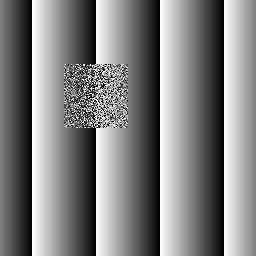
\includegraphics[width=0.24\textwidth]{images/2/00c_noise_wrapped.png}

\includegraphics[width=0.24\textwidth]{images/3/01a_noise_xy.png}

\includegraphics[width=0.24\textwidth]{images/3/01b_noise_yx.png}

\itkcaption[Itoh Phase Unwrapping Algorithm]{Noise-corrupted phase example ramps, unwrapped via the Itoh algorithm (\code{itk::ItohPhaseUnwrappingImageFilter}) in the horizontal then vertical directions (center) and in the vertical then horizontal directions (right).  The wrapped image (left) is reproduced for comparison.}
\label{fig:Itoh}
\end{figure}

\subsection{Phase Residues}

In order to predict when path-independent phase unwrapping is possible, it is necessary to introduce the concept of phase residues.  A residue charge is calculated for a 2x2 neighborhood of pixels and a given pair of dimensions, by summing the wrapped phase differences across a clockwise trajectory through the neighborhood and dividing the result by $2\pi$.\footnote{We here use the clockwise convention, as presented by Goldstein, et al \cite{Goldstein1988}.  However, as it is only the relative sign that is important for phase unwrapping, the clockwise/counter-clockwise convention makes no practical difference, so long as consistency is maintained.}  Effectively, this gives the number of positive discontinuities encountered less the number of negative discontinuities encountered (positive meaning that $2\pi$ would be added in order to remove it).

It has been proven that all phase residues have a value in the set $\left \{ -1, 0, 1\right \}$ \cite{Bone1991}.  Take the following minimal example (Figure~\ref{fig:Phase_Residues}):\footnote{For simplicity of calculation, the phase has been divided by $2\pi$ such that the range is from $(-0.5, 0.5]$ and the phase residues do not need to be rescaled.}

\begin{figure}[h]
\center
$\begin{matrix}

0.0 &  \rightarrow  & 0.3  &  \rightarrow & 0.3  &  \rightarrow  & 0.0 \\
\uparrow &  \odot  & \downarrow \uparrow &  & \downarrow \uparrow & \otimes & \downarrow \\
0.0 & \leftarrow   & -0.3 & \leftarrow  & -0.3 &  \leftarrow  & 0.0 \\

\end{matrix}$

\itkcaption[Phase_Residues]{Phase Residues.  Phase residues are calculated by summing the wrapped phase differences in a clockwise trajectory through a 2x2 neighborhood.  A positive residue ($\odot$) is noted in the leftmost neighborhood, a negative residue ($\otimes$) in the rightmost neighborhood, and no residue in the central neighborhood. }
\label{fig:Phase_Residues}
\end{figure}

The presence of one or more phase residues in a phase image denote path-dependent unwrapping.  In the above example, unwrapping along $(0,0) \rightarrow (1,0) \rightarrow (1,1)$ produces a value of $0.7$ for pixel $(1,1)$ ($-0.3 + 1.0 = 0.7)$, whereas unwrapping from $(0,0) \rightarrow (0,1) \rightarrow (1,1)$ produces a value of $-0.3$ because no phase wraps are encountered.\footnote{In accordance with ITK convention, the origin is taken to be the upper left corner of the image, and zero-indexing is used.}  Another useful result is that the wrapped line integral around a larger neighborhood yields the sum of the phase residues contained within that neighborhood.  In this example, the line integral is 0, which rightly reflects the presence of a single positive and a single negative residue.  Goldstein, et al \cite{Goldstein1988}, were the first to appreciate the significance of phase residues for path-dependency of phase unwrapping, by introducing the concept of residue `balancing' for 2D phase unwrapping.  They observed that, by defining branch cuts across which phase unwrapping was disallowed (either between residues of opposing sign or from a residue to the edge of the image), a subset of paths could be defined for which the wrapped line integral was zero (i.e., a subset of paths, none of which enclose an unbalanced residue).  Within this subset, any path taken will arrive at an identical unwrapped solution (to an arbitrary additive multiple of $2\pi$).

Appropriately balancing residues will ensure consistent, but not necessarily correct results \cite{Bone1991}.  All possible paths within a specific configuration yield the same result, to an additive multiple of $2\pi$.  However, results are not necessarily consistent between branch-cut configurations.  Figure~\ref{fig:Branch_Cuts} illustrates this point.  Two possible branch cut configurations are shown, each with one possible phase unwrapping path.  It is noteworthy that the values of pixels $(1,1)$ and $(2,1)$ differ between the two configurations.

\begin{figure}[h]
\center

\begin{tabular}{@{}c@{}}
  
  $\begin{matrix}

0.0 &  \rightarrow  & 0.3  &  \rightarrow & 0.3  &  \rightarrow  & 0.0 \\
 & \odot & \textrm{---} &  & \textrm{---} & \otimes & \downarrow \\
0.0 & \leftarrow   & -0.3 & \leftarrow  & -0.3 &  \leftarrow  & 0.0 \\

\end{matrix}$

\\
\small (a)

\end{tabular}

\vspace{\floatsep}

\begin{tabular}{@{}c@{}}


$\begin{matrix}

0.0 &  \rightarrow  & 0.3  &  & 0.3  &  \rightarrow  & 0.0 \\
\uparrow & \odot & \downarrow &  & \uparrow & \otimes & \downarrow \\
0.0 & |   & 0.7 & \rightarrow  & 0.7 &  |  & 0.0 \\

\end{matrix}$

\\
\small (b)

\end{tabular}


\itkcaption[Branch_Cuts]{Branch Cut Configurations.  The above example demonstrates two possible branch cut configurations.  Configuration (a) connects residues of opposing sign to one another.  Configuration (b) connects each residue to the image border.  For each configuration, one possible unwrapping path is demonstrated.  `---' and `$|$' represent vertical and horizontal branch cuts, respectively; arrows represent the path of phase unwrapping.}
\label{fig:Branch_Cuts}
\end{figure}

It should also be noted that the branch cutting theory so far discussed in this section is specific to two dimensional phase unwrapping.  An extension of the branch cutting concept to three dimensions has been proposed \cite{Huntley2001}, which requires phase residues to be calculated with respect to each pair of dimensions (xy, xz, yz).  To our knowledge, the branch cutting method has not been extended to higher dimensions.  We have included a discussion of residues for completeness, and because we believe that the concepts are essential to the understanding of path dependence.  However, as our interest in this submission is with phase unwrapping filters that may be implimented over images of arbitrary dimension, no branch cutting algorithms have been included.

Phase residues may be calculated using the \code{itk::PhaseResidueImageFilter} class (defined in \code{itkPhaseResidueImageFilter.h} (Figure~\ref{fig:Phase_Residues_Noise_Patch}).  The filter inherits from \code{itk::PhaseImageToImageFilter}, and uses the \code{Wrap()} method to calculate phase residues as described above.  Note that, due to the theoretical limitations described above, the filter only has a clear physical significance for 2D images.

\begin{figure}[h]
\center
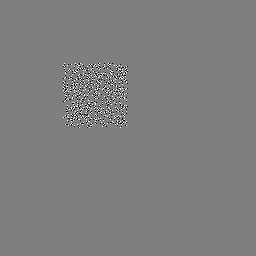
\includegraphics[width=0.24\textwidth]{images/3/02a_residue.png}

\itkcaption[Phase_Residues_Noise_Patch]{Phase residues are calculated for the noise-corrupted phase ramp example using the \code{itk::PhaseResidueImageFilter} class.}
\label{fig:Phase_Residues_Noise_Patch}
\end{figure}

\subsection{The Helmholtz Decomposition}

Given a vector field $v$, if there exists some $A$ such that $v = \nabla \times A$, then $A$ is called the `vector potential' of $v$.  Given that the divergence of the curl of any vector field is the zero vector, $v$ must therefore be entirely rotational (i.e., non-conservative):

\begin{equation}
\label{eqn:Div_Curl_Identity}
\nabla \cdot v = \nabla \cdot ( \nabla \times A ) = 0
\end{equation}

Likewise, if there exists some $\psi$ such that $v = \nabla \psi$, then $\psi$ is called the `scalar potential' of $v$.  Given that the curl of the gradient of any scalar field is zero, $v$ must therefore be entirely irrotational (i.e., conservative):

\begin{equation}
\label{eqn:Curl_Grad_Identity}
\nabla \times v = \nabla \times ( \nabla \psi ) = 0
\end{equation}

In the general case, $A$ and $\psi$ cannot be found (that is, the general case of a vector field need not be entirely rotational or irrotational).  However, the Helmholtz Decomposition states that a vector field can be decomposed into rotational and irrotational components as the sum of scalar and vector potentials:

\begin{equation}
\label{eqn:Helmholtz}
v = - \nabla \psi + \nabla \times A
\end{equation}

In the context of phase unwrapping, the Helmholtz decomposition has specific implications for path dependence.  In particular, the `path-dependent' contribution is contained entirely within the rotational component, and the `path-independent' contribution within the irrotational component.  The irrotational and rotational components of the noise-corrupted phase ramp are shown in the left and right panels of Figure~\ref{fig:Helmholtz_Decomposition}.  Note in the irrotational component that corruption of the original phase extends beyond the patch of noise itself, though there are no ambiguities.

\begin{figure}
\center

\includegraphics[width=0.24\textwidth]{images/3/02b_irrotational.png}
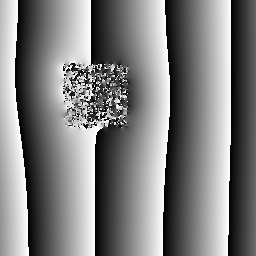
\includegraphics[width=0.24\textwidth]{images/3/02c_rotational.png}

\itkcaption[Helmholtz_Decomposition]{The \code{itk:HelmholtzDecompositionImageFilter} classe, applied to the noise-corrupted phase ramp example.  The left panel is the irrotational (curl-free) component, and the right panel is the rotational (divergence-free) component.}
\label{fig:Helmholtz_Decomposition}
\end{figure}

The Helmholtz Decomposition is provided in the \code{itk::HelmholtzDecompositionImageFilter} class (defined in \code{itkHelmholtzDecompositionImageFilter.h}), which inherits from \code{itk::PhaseImageToImagefilter}.  The irrotational and rotational components may be retrieved through the \code{GetRotational()} and \code{GetIrrotational()} methods, respectively.

The implementation of \code{itk::HelmholtzDecompositionImageFilter} takes advantage of the fact that the irrotational component is equivalent to the unweighted, least squares solution (\code{itk::DCTPhaseUnwrappingImageFilter}, discussed in a later section), re-wrapped into the range $(-\pi, \pi]$.  The rotational component may then be obtained by subtracting the irrotational component from the original wrapped phase, and re-wrapping the result.

\subsection{Phase Derivative Variance}

It addition to phase residues, it is also useful to consider continuous measures of phase quality, of which the phase derivative variance is the most commonly used.  Phase derivative variance $\sigma$ in a single dimension $d$ is the sum of squared differences of the local wrapped phase gradients ($\Delta \phi_{i}$) and the mean wrapped phase gradient ($\overline{ \Delta \phi }$, Equation~\ref{eqn:PhaseDerivativeVariance}). 

\begin{equation}
\label{eqn:PhaseDerivativeVariance}
\sigma_d = \sum_i{  \left( \Delta \phi_{i} - \overline{ \Delta \phi }     \right)^2  }
\end{equation}

The total phase derivative variance can then be found by dividing the sum of the root variance in each dimension by the square of the one-sided length of the neighborhood $k$ (Equation~\ref{eqn:PhaseDerivativeVarianceTotal}).  Phase derivative variance is a convenient measure of phase quality because it (a) is easily generalized to arbitrary dimension and (b) can be computed entirely from the phase data itself.

\begin{equation}
\label{eqn:PhaseDerivativeVarianceTotal}
\frac{ \sum_d { \sqrt{ \sigma_d } }  }{ k^2 }
\end{equation}

Phase derivative variance is an inverse measure of phase quality; i.e., a large phase derivative variance is indicative of low phase quality.  In order to be used as a quality metric, phase derivative variance is typically rescaled into the range $[0,1]$ and multiplied by $-1$, such that brighter pixels represent higher phase quality.  This is the default behavior of \code{itk::PhaseDerivativeVarianceImageFilter}.  The un-normalized phase derivative variance can be obtained by setting \code{SetNormalize(false)}.  The rescaled phase derivative variance image for the noise-corrupted phase ramp is shown in Figure~\ref{fig:Phase_Derivative_Variance}.

Note that the patch of noise can be clearly identified in the original wrapped image, the phase residue image, the phase derivative variance image, and the rotational component of the Helmholtz decomposition.

\begin{figure}[h]
\center
\fbox{ 
\includegraphics[width=0.24\textwidth]{images/3/02d_quality.png} }

\itkcaption[Phase_Derivative_Variance]{Phase Derivative Variance.  Rescaled phase derivative variance for the noise-corrupted phase ramp, computed with \code{itk::PhaseDerivativeVarianceImageFilter}.  The patch of noise can be clearly identified as a region of low image quality.  Note that a thin black border has been added in order to allow visualization of the edge of the image.}
\label{fig:Phase_Derivative_Variance}
\end{figure}

\clearpage
\input{"includes/Phase Unwrapping"}
\clearpage
\section{Clinical Examples}

\subsection{Susceptibility Weighted Imaging (SWI) of the Brain}

SWI is an MR technique used to enhance microhemorrhage and calcification in the brain.  This sequence exploits distortion of the MR field by paramagnetic (e.g., deoxyhemoglobin) and diamagnetic (e.g., dystrophic calcification) compounds, requiring the combination of magnitude and unwrapped phase images.  An example of a wrapped phase image obtained from an SWI sequence is shown in Figure~\ref{fig:SWI}.  The image is an axial slice taken through the brain.

\begin{figure}[h]
\center

\includegraphics[width=0.24\textwidth]{images/input/wrapped_swi.png}

\itkcaption[SWI of the Brain]{Wrapped phase data from SWI of the brain.}
\label{fig:SWI}
\end{figure}

The \code{itk::PhaseResidueImageFilter}, \code{itk::PhaseDerivativeVarianceImageFilter}, and \code{itk::HelmholtzDecompositionImageFilter} classes are demonstrated for the SWI data in Figure~\ref{fig:Exploring_SWI_Data}.  The residues are almost entirely restricted to the region outside the skull.  The Helmholtz decomposition shows that, as expected, most of the information in the low-quality, residue-rich region outside the skull is due to the rotational contribution, whereas most of the upward spike in phase in the anterior brain tissue is due to the irrotational contribution.  The phase derivative variance image shows high quality phase data within the brain tissue and low quality data otherwise.

\begin{figure}[h]
\center

\includegraphics[width=0.24\textwidth]{images/swi/03a_residue.png}

\includegraphics[width=0.24\textwidth]{images/swi/03b_irrotational.png}

\includegraphics[width=0.24\textwidth]{images/swi/03c_rotational.png}

\includegraphics[width=0.24\textwidth]{images/swi/03d_quality.png}

\itkcaption[Exploring_SWI_Data]{Phase data from susceptibility weighted imaging of the brain.  From left to right: residues; irrotational component; rotational component; normalized phase derivative variance.}
\label{fig:Exploring_SWI_Data}
\end{figure}


\begin{figure}
\center

\includegraphics[width=0.32\textwidth]{images/input/wrapped_swi.png}

\includegraphics[width=0.32\textwidth]{images/swi/03e_qg_unwrap.png}

\includegraphics[width=0.32\textwidth]{images/swi/03f_dct_unwrap.png}

\itkcaption[Unwrapped Susceptibility Data]{Phase data from susceptibility weighted imaging of the brain.  Presented are the original image (left), the result of the quality-guided phase unwrapping algorithm (\code{itk:QualityGuidedPhaseUnwrappingImageFilter}, center), and of the DCT phase unwrapping algorithm (\code{itk:DCTPhaseUnwrappingImageFilter}, right).}
\label{fig:SWI_Unwrap}
\end{figure}

We now present the results of the Quality-Guided and DCT phase unwrapping algorithms (Figure~\ref{fig:SWI_Unwrap}).  The quality-guided approach (center) appears to correctly unwrap through the vast majority of the brain matter.  Upon close inspection, however, small areas of `roughness' are noted in regions of the brain matter closely correlating with residue pairs and clusters in the original image, presumably due to local noise (Figure~\ref{fig:SWI_Quality_Inset}).  The minimum $L^2$-norm approach gives a smooth result throughout.


\begin{figure}[h]
\center

\begin{tikzpicture}
    \node[anchor=south west,inner sep=0] (image) at (0,0) {
\includegraphics[trim = 70px 260px 70px 65px, clip, width=0.49 \textwidth]{images/swi/03a_residue.png}};
    \begin{scope}[x={(image.south east)},y={(image.north west)}]
        \draw [red] (0.5,0.675) ellipse (0.75cm and 0.5cm);
        \draw [red] (0.5,0.15) ellipse (0.75cm and 0.5cm);
    \end{scope}
\end{tikzpicture}

\begin{tikzpicture}
    \node[anchor=south west,inner sep=0] (image) at (0,0) {
\includegraphics[trim = 70px 260px 70px 65px, clip, width=0.49 \textwidth]{images/swi/03e_qg_unwrap.png}};
    \begin{scope}[x={(image.south east)},y={(image.north west)}]
        \draw [red] (0.5,0.675) ellipse (0.75cm and 0.5cm);
        \draw [red] (0.5,0.15) ellipse (0.75cm and 0.5cm);
    \end{scope}
\end{tikzpicture}


\itkcaption[SWI_Quality_Inset]{ Inset of the SWI residue (upper) and quality-guided phase unwrapped (lower) images.  Note the regions of minor discontinuity in the unwrapped image in regions corresponding to pairs/clusters of residues. }
\label{fig:SWI_Quality_Inset}
\end{figure}

A cross-section through the vertical centerline of the image is plotted in Figure~\ref{fig:SWI_Congruence}.  The quality-guided approach gives a congruent result throughout.  The DCT algorithm follows the gradient closely, but underestimates the phase.

\begin{figure}[h]
\center

\begin{tikzpicture}
    \node[anchor=south west,inner sep=0] (image) at (0,0) {
\includegraphics[width=0.28\textwidth]{images/input/wrapped_swi.png}};
    \begin{scope}[x={(image.south east)},y={(image.north west)}]
        \draw[red,ultra thick] (0.5,0) -- (0.5,1);
    \end{scope}
\end{tikzpicture}
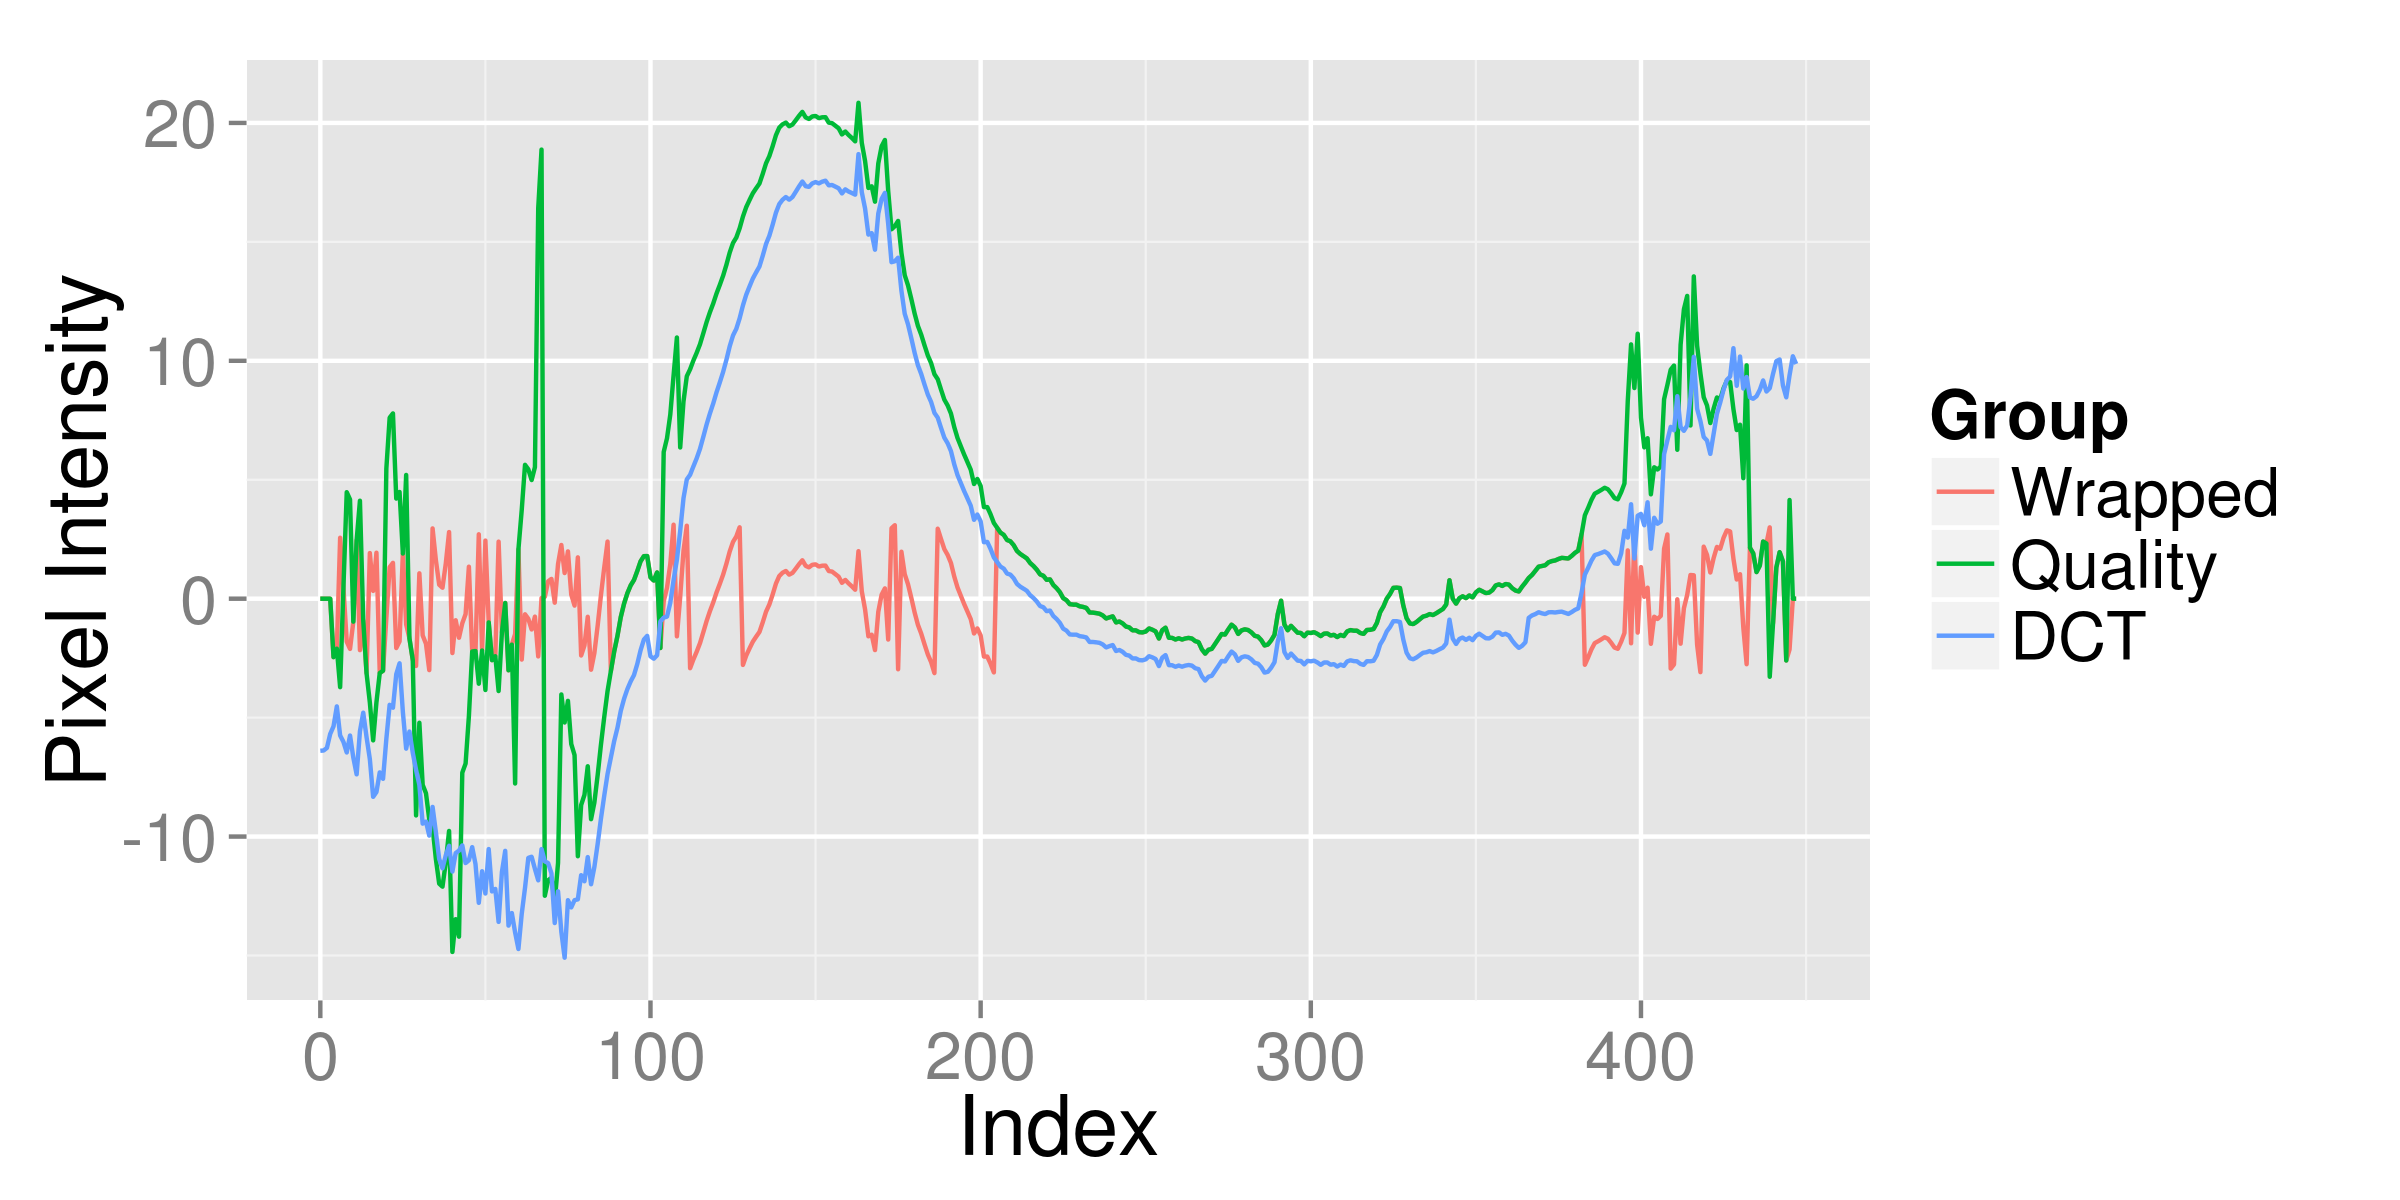
\includegraphics[width=0.71\textwidth]{images/swi/congruence.png}
\itkcaption[SWI_Congruence]{Congruence in SWI Data.  The pixel intensities from the vertical centerline of the SWI image are plotted for the unwrapped and original SWI data.  Note that the quality-guided approach is congruent throughout, but contains a discontinuity.  The DCT approach is smooth throughout, but is not congruent.}
\label{fig:SWI_Congruence}
\end{figure}

\newpage
\subsection{Harmonic Phase (HARP) Imaging of the Heart}

Spatial modulation of magnetization (SPAMM) is an MRI pulse sequence which modulates the signal magnitude in a periodic fashion across the plane of the image, resulting in lines of decreased signal \cite{Axel1989}.  The phase of this magnetude modulation is a material property of the tissue, and as such remains constant over time and with movement.  Therefore, tag lines laid down in the heart at end diastole will deform along with the heart during contraction, and so can be used to visualize cardiac deformation (Figure~\ref{fig:SPAMM}).

\begin{figure}[h]
\center
% left bottom right top
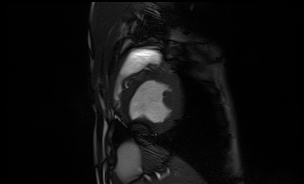
\includegraphics[trim = 100px 40px 110px 34px, clip, width=0.24\textwidth]{images/canine/ssfp_ed.png}

\includegraphics[trim = 100px 50px 110px 30px, clip, width=0.24\textwidth]{images/canine/spamm_ed.png}

\includegraphics[trim = 100px 50px 110px 30px, clip, width=0.24\textwidth]{images/input/wrapped_harp_ed.png} \\
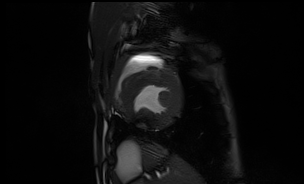
\includegraphics[trim = 100px 40px 110px 34px, clip, width=0.24\textwidth]{images/canine/ssfp_es.png}

\includegraphics[trim = 100px 50px 110px 30px, clip, width=0.24\textwidth]{images/canine/spamm_es.png}

\includegraphics[trim = 100px 50px 110px 30px, clip, width=0.24\textwidth]{images/input/wrapped_harp.png}

\itkcaption[SPAMM]{Balanced steady state free precession (SSFP) images (left) are shown alongside corresponding tagged SPAMM (center) and HARP (right) images in a canine subject.  Shown are short axis, mid-ventricular images.  The upper panels were acquired at end diastole (no contraction); the lower panels were acquired at end systole (maximal contraction).  Note that circumferential shortening and radial thickening of the myocardium is apparent by observing the deformation of the tag lines.}
\label{fig:SPAMM}
\end{figure}

Harmonic phase analysis is an automated technique for calculating strain from tagged MR images \cite{Osman1999a}.  Cardiac strain is calculated from ``HARP'' images, which are the result of filtering in the Fourier domain.  Many versions of this algorithm require that these images be unwrapped prior to strain calculation \cite{Venkatesh2010, Venkatesh2011}.  SSFP, SPAMM, and HARP images at end systole and end diastole are shown in Figure~\ref{fig:SPAMM}.

The \code{itk::PhaseResidueImageFilter}, \code{itk::PhaseDerivativeVarianceImageFilter}, and \code{itk::HelmholtzDecompositionImageFilter} classes are demonstrated for the HARP data in Figure~\ref{fig:Exploring_HARP_Data}.

\begin{figure}[h]
\center

\includegraphics[trim = 100px 50px 110px 30px, clip, width=0.24\textwidth]{images/harp/03a_residue.png}

\includegraphics[trim = 100px 50px 110px 30px, clip, width=0.24\textwidth]{images/harp/03d_quality.png}

\includegraphics[trim = 100px 50px 110px 30px, clip, width=0.24\textwidth]{images/harp/03b_irrotational.png}

\includegraphics[trim = 100px 50px 110px 30px, clip, width=0.24\textwidth]{images/harp/03c_rotational.png}

\itkcaption[Exploring_HARP_Data]{Phase data from HARP imaging of the heart.  From left to right: residues, phase derivative variance, irrotational component, and rotational component.}
\label{fig:Exploring_HARP_Data}
\end{figure}

We now present the results of the Quality-Guided and DCT phase unwrapping algorithms (Figure~\ref{fig:HARP_Unwrap}).  From the unwrapped image it is clear that the quality-guided approach gives an unsatisfactory result, with phase wraps passing through the myocardial wall.  The result of the DCT approach is smooth, but otherwise difficult to evaluate by looking at the image directly.

\begin{figure}[h]
\center

\includegraphics[trim = 100px 50px 110px 30px, clip, width=0.32\textwidth]{images/input/wrapped_harp.png}

\includegraphics[trim = 100px 50px 110px 30px, clip, width=0.32\textwidth]{images/harp/03e_qg_unwrap.png}

\includegraphics[trim = 100px 50px 110px 30px, clip, width=0.32\textwidth]{images/harp/03f_dct_unwrap.png}

\itkcaption[Unwrapped HARP Data]{Results of the phase unwrapping algorithms.  Quality guided (center) and DCT (right) results are presented.  The original wrapped image is also presented (left) for comparison.}
\label{fig:HARP_Unwrap}
\end{figure}

A plot through the centerline of the image shows that the DCT approach is also unsatisfactory, as the gradient differs considerably from that of the wrapped phase input.

\begin{figure}[h]
\center
\begin{tikzpicture}
    \node[anchor=south west,inner sep=0] (image) at (0,0) {
\includegraphics[trim = 100px 50px 110px 30px, clip, width=0.29\textwidth]{images/input/wrapped_harp.png}};
    \begin{scope}[x={(image.south east)},y={(image.north west)}]
        \draw[red,ultra thick] (0.5,0) -- (0.5,1);
    \end{scope}
\end{tikzpicture}
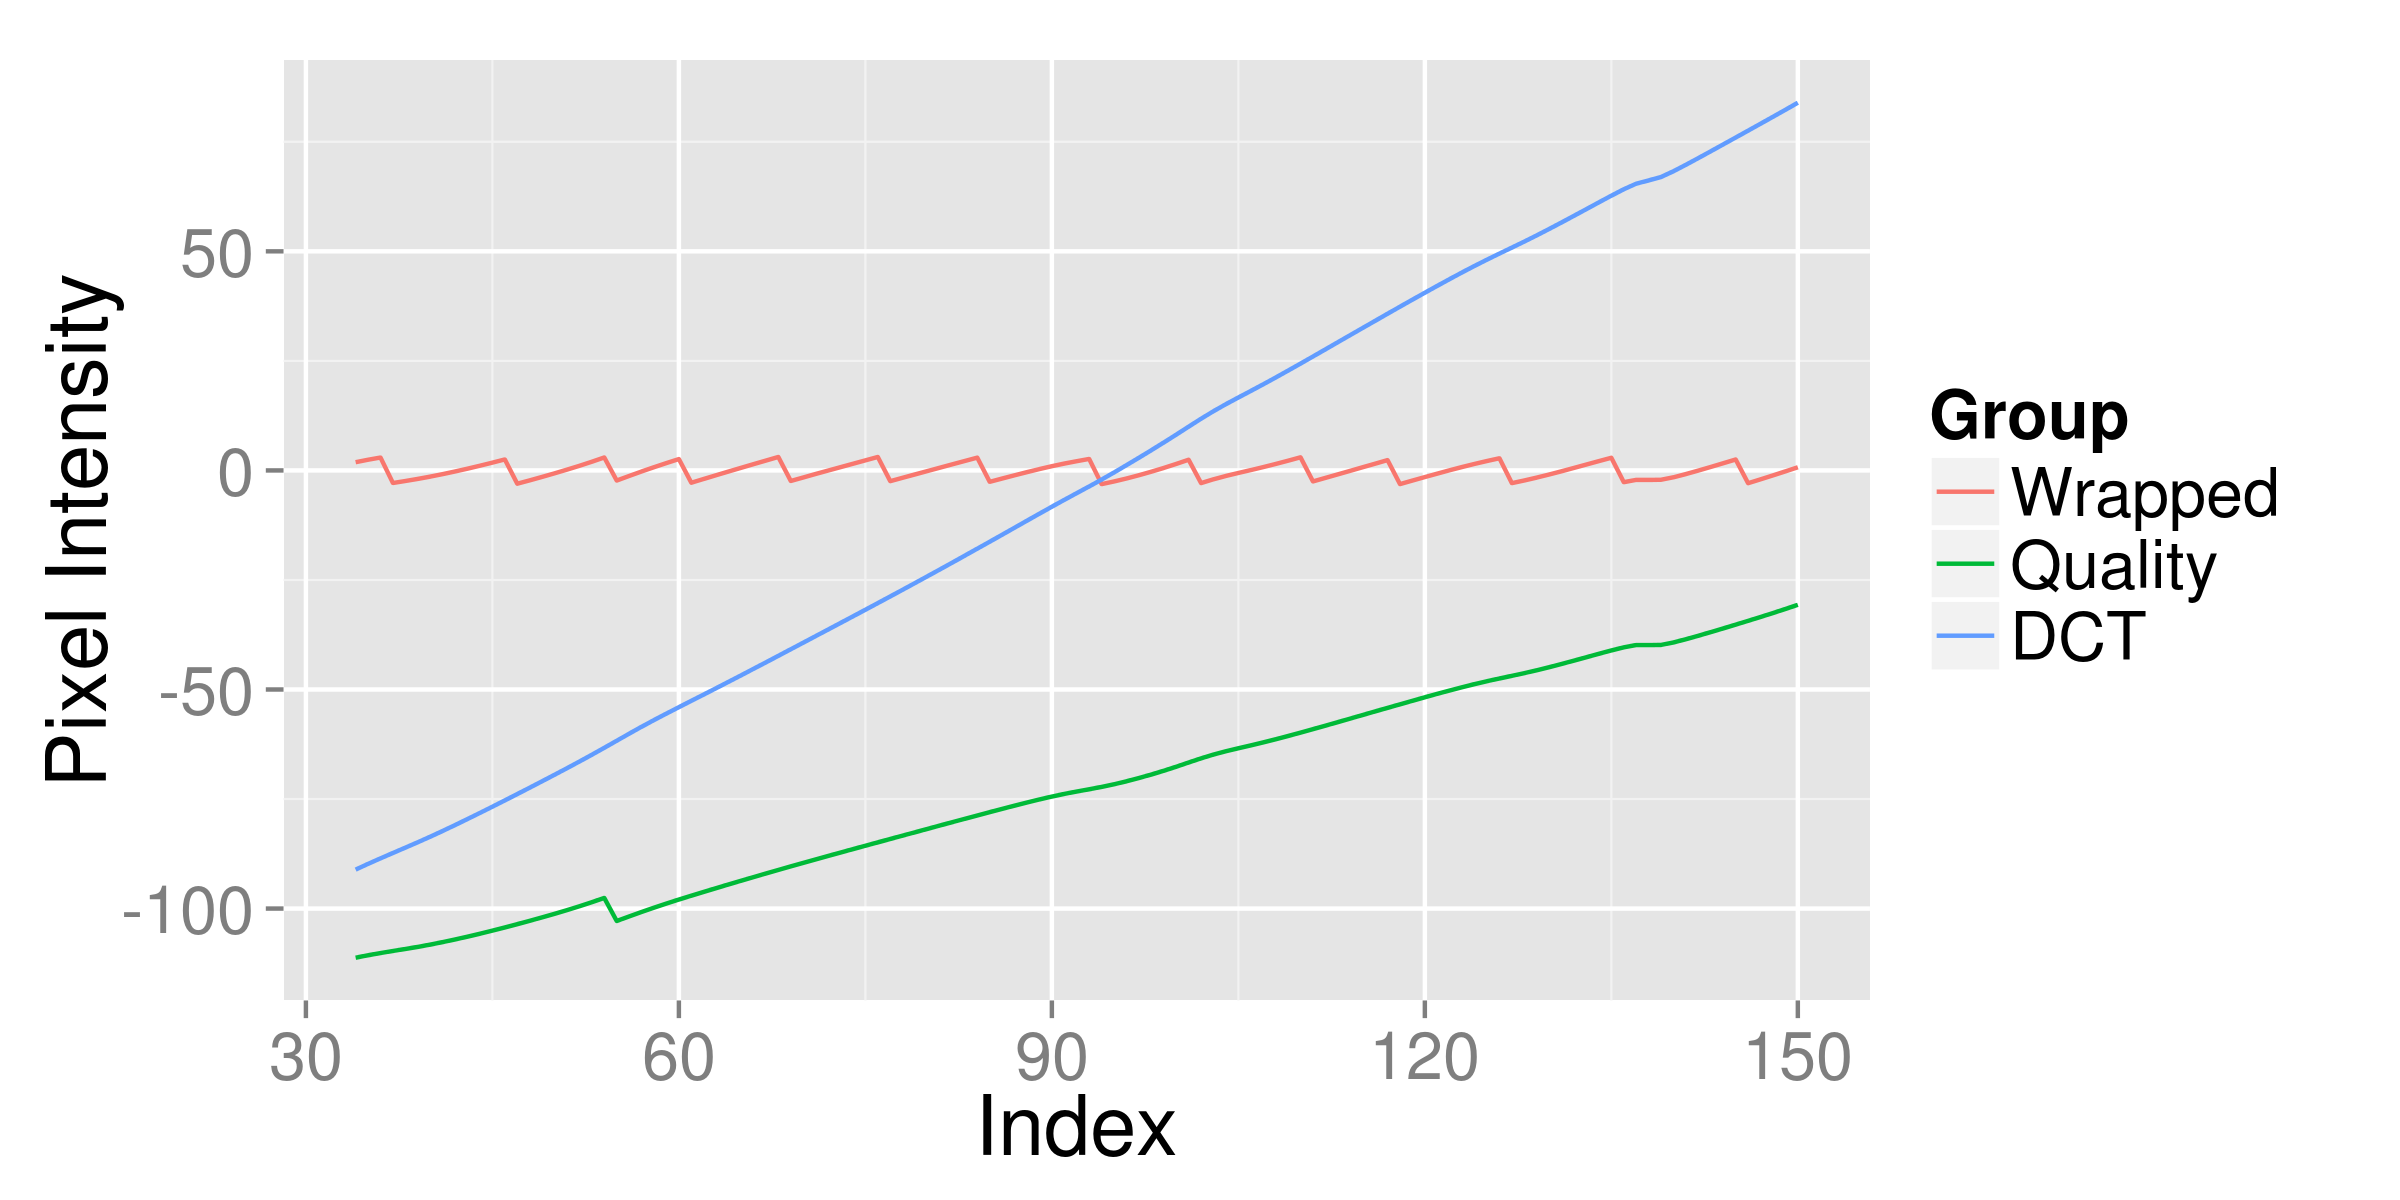
\includegraphics[width=0.70\textwidth]{images/harp/congruence.png}
\itkcaption[HARP_Congruence]{Congruence in HARP Data.  The pixel intensities from the vertical centerline of the HARP image are plotted for the unwrapped and original HARP data.  Note that the quality-guided approach is congruent throughout, but contains a discontinuity.  The DCT approach is smooth throughout, but is not congruent.}
\label{fig:HARP_Congruence}
\end{figure}

\subsection{A Note on Computational Speed}

The \code{itk::TimeProbe} class was used to measure the excecution time for the quality-guided and $L^2$-norm implementations on a single-processor Ubuntu 12.0.2 virtual machine with 4GB of memory.  For the SWI data, the quality-guided and $L^2$-norm approaches took $1.14$ and $0.75s$, respectively.  For the HARP data, the quality-guided and $L^2$-norm approaches took $0.40$ and $0.27s$, respectively.  Successive runs differed by less than 0.01s.  Therefore, the quality-guided approach took slighly less than twice as long to execute, though this difference may be insignificant for many applications.  Importantly, execution times are expected to grow linearly with input size for the quality-guided approach and by $O(n \log n)$ for the $L^2$-norm approach.  The quality-guided approach could be sped up by allowing for a mask that would prevent the unwrapping of pixels outside the area of interest and the DCT approach could be sped up by taking advantage of multithreading.  However, as has been shown, for some applications it may be necessary to incorporate the DCT algorithm into an iterative algorithm such as preconditioned conjugate gradient weighted $L^2$-norm in order to achieve satisfactory results, which could negate advantages gained through multithreading.
\clearpage
\section{Conclusions and Future Directions}

ITK is a large and powerful framework for medical (and general) image processing.  However, the lack of filters for understanding, manipulating, and unwrapping phase data is a current limitation of the library.  We have here presented an ITK module which we hope will begin to bridge that gap.  The two most significant contributions are the \code{itk::QualityGuidedPhaseUnwrappingImageFilter} and \code{itk::DCTPhaseUnwrappingImageFilter} classes, which implement efficient $n$-dimensional unwrapping algorithms.  The quality-guided approach has the advantage of giving a result that is congruent to the input.  Moreover, this approach avoids low-quality phase data, given an adequate quality map.  The unweighted $L^2$-norm approach has the advantage of giving a smooth result throughout, but is not congruent with the input and weights all pixels equally regardless of quality.

These algorithms both gave servicable results when presented with the SWI data, which had few residues within the region of interest, and in which the low quality data was largely relegated to the periphery.  However, both algorithms failed to produce an adequate result when presented with the more difficult HARP image.  In the case of the quality-guided approach, this is likely due to the inadequacy of phase derivative variance as a quality map, because in HARP images phase varies quite smoothly even in regions where there is little to no signal.  In the case of the DCT algorithm, this is likely because the region of interest is relatively small compared to the image as a whole.

In the future, it would be of great benefit to allow for other quality maps (such as maximum phase gradient, pseudocorrelation, and user-defined masks) in addition to phase derivative variance.  This would allow for finer control over the path the algorithm takes in the case of difficult cases such as HARP images.  Additionally, it would be of benefit to implement a weighted $L^2$-norm method, so that the DCT approach could also exclude low-quality or uninteresting regions.  Weighted $L^2$-norm phase unwrapping algorithms have been described which iteratively apply unweighted algorithms to weighted wrapped phase Laplacians.  The preconditioned conjugate gradient (PCG) approach in particular makes use of this method \cite{Ghiglia1998}, and would be an important next step in the development of this module.

This submission has also described \code{itk::DCTImageFilter} and \code{itk::DCTPoissonSolverImageFilter}, which are efficient implementations of general-purpose utilities important in image compression, gradient image editing, and phase unwrapping.  The former is a simple wrapper to the FFTW library, allowing for the discrete cosine transform to be integrated into an ITK pipeline.  The latter makes use of the DCT class to recover an image from its Laplacian.  We refer the interested reader to the appendices for a proper discussion.
\clearpage

\appendix

\section{Laplace's Equation}

The Laplacian operator, $\Delta$, is defined for an $n$-dimensional function as the sum of its unmixed partial second derivatives (Equation~\ref{eqn:LaplacianOperator}):

\begin{equation}
\label{eqn:LaplacianOperator}
\Delta f = \nabla^2f = \sum_{i=1}^n \frac{\delta^2f}{\delta x_i^2}
\end{equation}

In the two-dimensional case, this takes the following familiar form (Equation~\ref{eqn:2DLaplacianOperator}):

\begin{equation}
\label{eqn:2DLaplacianOperator}
\Delta f = \frac{\delta^2 f}{\delta x^2} + \frac{\delta^2 f}{\delta y^2}
\end{equation}

In the special case where $\Delta f = 0$, this is known as Laplace's Equation. The discrete Laplacian may be approximated via simple second differences.  The one-dimensional second-difference operator $\begin{matrix}[1 & -2 & 1]\end{matrix}$ may be taken successively in each image dimension to produce a Laplacian image.  In the two-dimensional case, the discrete Laplacian operator is computed as follows:

\begin{equation}
\label{eqn:2DDiscreteLaplacianOperator}
\begin{matrix}
0 $ 1 $ 0 \\
1 $ -4 $ 1 \\
0 $ 1 $ 0
\end{matrix}
\end{equation}

In ITK, the discrete Laplacian operator is provided in the \doxygen{LaplacianOperator} class, and is applied to an image using the \doxygen{LaplacianImageFilter} class.  Laplace's equation can be solved efficiently by means of the discrete cosine transform (DCT) \cite{Ghiglia1998}.  In particular, the original image $f$ can be recovered by taking the forward DCT of the Laplacian image $\Delta f$, applying a pixelwise modulation, and taking the reverse DCT on the result (Equation~\ref{eqn:DCTPoisson}).  In this equation, $n$ is the dimension of the image, $S_n$ is the number of pixels across the image in direction $d$, and $i_n$ is the pixel index in direction $n$.

\begin{equation}
\label{eqn:DCTPoisson}
f = DCT^{-1} \left \{\frac{\displaystyle DCT \left \{ \Delta f \right \}}{\displaystyle \sum_{n=0}^{N-1} 2 \cos \left( \frac{\displaystyle \pi i_n}{\displaystyle S_n} \right) -2N} \right \}
\end{equation}

It is possible to formulate the problem in such a way that it can be solved with either the fast Fourier transform (FFT), discrete sine transform (DST), or discrete cosine transform (DCT).  The specifics of each implementation differ primarily in the steps that must be undertaken to satisfy Neumann boundary conditions.  In order to be solved with the FFT, for instance, the Laplacian must be reflected to the left and upwards (Figure ~\ref{fig:Reflection}).  The DCT (also known as the `even' or `real-to-real' transform), however, is performed on one half of an implicitly reflected matrix, obviating the reflection step.  Though this difference is likely negligible for an isolated 2D calculation, use of the DCT could significantly reduce memory and processing requirements when applied iteratively or to higher dimensional data.  For this reason, the DCT is prefered if available.

\begin{figure}[h]
\center
\scalebox{-1}[-1]{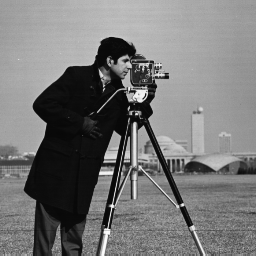
\includegraphics[width=0.25\textwidth]{images/appendix/cameraman.png}}
\hspace{-6px}
\scalebox{1}[-1]{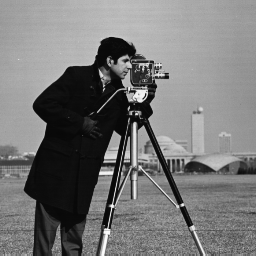
\includegraphics[width=0.25\textwidth]{images/appendix/cameraman.png}} \\
\vspace{-2px}
\scalebox{-1}[1]{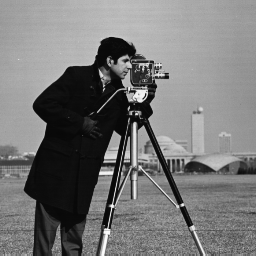
\includegraphics[width=0.25\textwidth]{images/appendix/cameraman.png}}
\hspace{-6px}
\scalebox{1}[1]{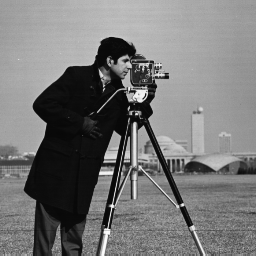
\includegraphics[width=0.25\textwidth]{images/appendix/cameraman.png}}
\itkcaption[Reflection]{The ``cameraman'' test image, reflected to the left and upwards to satisfy Neumann boundary conditions.}
\label{fig:Reflection}
\end{figure}

\section{Implementation and Usage}

\subsection{Discrete Cosine Transform}

FFTW (the `Fastest Fourier Transform in the West' \cite{Frigo2005}) is a library in the C programming language, which can be made available by building ITK with the CMake variable \code{ITK\_USE\_FFTWF} or \code{ITK\_USE\_FFTWD} (single and double precision floating point, respectively) to \code{ON}.  FFTW provides a wide selection of efficient discrete transforms, including DCT types I--IV (corresponding to `\code{kind}s' \code{REDFT00}, \code{REDFT10}, \code{REDFT01}, and \code{REDFT11}, respectively).  These plans differ practically from one another in terms of inverse transforms and normalization procedures (\code{REDFT00} and \code{REDFT11} are inverses of themselves, whereas \code{REDFT10} and \code{REDFT01} are inverses of each other).  In particular, \code{REDFT10} and \code{REDFT01} are known as `the' forward and reverse DCT, respectively.  A real-to-real plan is constructed according to the following function definition:

\small
\begin{verbatim}
fftw_plan fftw_plan_r2r(int rank, const int *n, double *in, double *out,
                             const fftw_r2r_kind *kind, unsigned flags);
\end{verbatim}
\normalsize

\code{int rank} refers to the image dimension; \code{const int *n} to an array indicating the size in each dimension; \code{double *in} and \code{double *out} to input and output arrays allocated using \code{fftw\_malloc}, \code{const fftw\_r2r\_kind *kind} to the type of transform that should be performed in each dimension, and \code{unsigned flags} to instructions concerning numerical precision.  The \code{itk::Image} buffers are assigned to the input and output arrays using the \code{GetBufferPointer()} method.  Each element of the \code{const fftw\_r2r\_kind} array is set to \code{FFTW\_REDFT01} in the case of the forward transform and \code{FFTW\_REDFT10} in the case of the inverse transform.  The transform direction can be specified at the level of the itk class using the \code{TransformDirection()} method.  Because FFTW returns an unnormalized transform, the image is divided by \code{numpix*pow(2, TInputImage::ImageDimension)} in the case of the inverse transform.

The provided class \code{itk::DCTImageFilter}, which inherits from \code{itk::ImageToImageFilter}, provides a simple, templeted interface to the \code{REDFT01} and \code{REDFT10} plans.  The following minimal example code demonstrates definition, instantiation, and usage of the class, and Figure~\ref{fig:DCT} illustrates a simple low-pass DCT filtering example (source code provided).\footnote{Note that all images have been linearly rescaled (except for transforms, which have been logarithmically rescaled) for visualization purposes.}

\small
\begin{verbatim}
typedef itk::DCTImageFilter< WorkImageType, WorkImageType > DCTType;
DCTType::Pointer dct = DCTType::New();
dct->SetInput( reader->GetOutput() );
dct->SetTransformDirection( DCTType::Forward );
dct->Update();
\end{verbatim}
\normalsize

\begin{figure}
\center
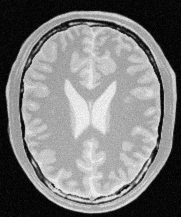
\includegraphics[width=0.24\textwidth]{images/appendix/brain.png}

\includegraphics[width=0.24\textwidth]{images/appendix/dct.png}
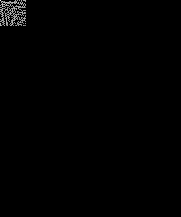
\includegraphics[width=0.24\textwidth]{images/appendix/dctFiltered.png}

\includegraphics[width=0.24\textwidth]{images/appendix/filtered.png}
\itkcaption[Reflection]{Simple demonstration of low-pass DCT filtering.  From left to right are the input image, the DCT transform, the masked transform, and the output image.}
\label{fig:DCT}
\end{figure}

\subsection{Poisson Solver}

The \code{itk::DCTPoissonSolver} class transforms the input, applies a modulation, and reverse transforms back into the image domain, as described in Equation~\ref{eqn:DCTPoisson}.  The following minimal example demonstrates definition, instantiation, and usage of the \code{itk::DCTPoissonSolverImageFilter} class.

\small
\begin{verbatim}
typedef itk::DCTPoissonSolverImageFilter< WorkImageType, WorkImageType >   PoissonType;
PoissonType::Pointer solver = PoissonType::New();
solver->SetInput( laplacian->GetOutput() );
solver->Update();
\end{verbatim}
\normalsize

\begin{figure}
\center
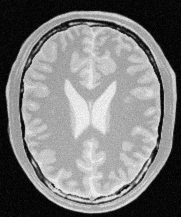
\includegraphics[width=0.32\textwidth]{images/appendix/brain.png}

\includegraphics[width=0.32\textwidth]{images/appendix/laplacian.png}

\includegraphics[width=0.32\textwidth]{images/appendix/solution.png}
\itkcaption[Laplacian]{The original (left) and Laplacian (right) images for an axial CT slice through the brain.}
\label{fig:Laplacian}
\end{figure}

Figure~\ref{fig:Laplacian} shows an example of an image of the brain, its Laplacian, and the solution of the Laplacian.  In the rescaled image, the solution appears to match exactly the input image.  However, by plotting the vertical centerline of each image (Figure~\ref{fig:Additive}), we see that the input and output differ by an additive constant of $\sim123.7$, as is expected from any integration procedure.

\begin{figure}
\center
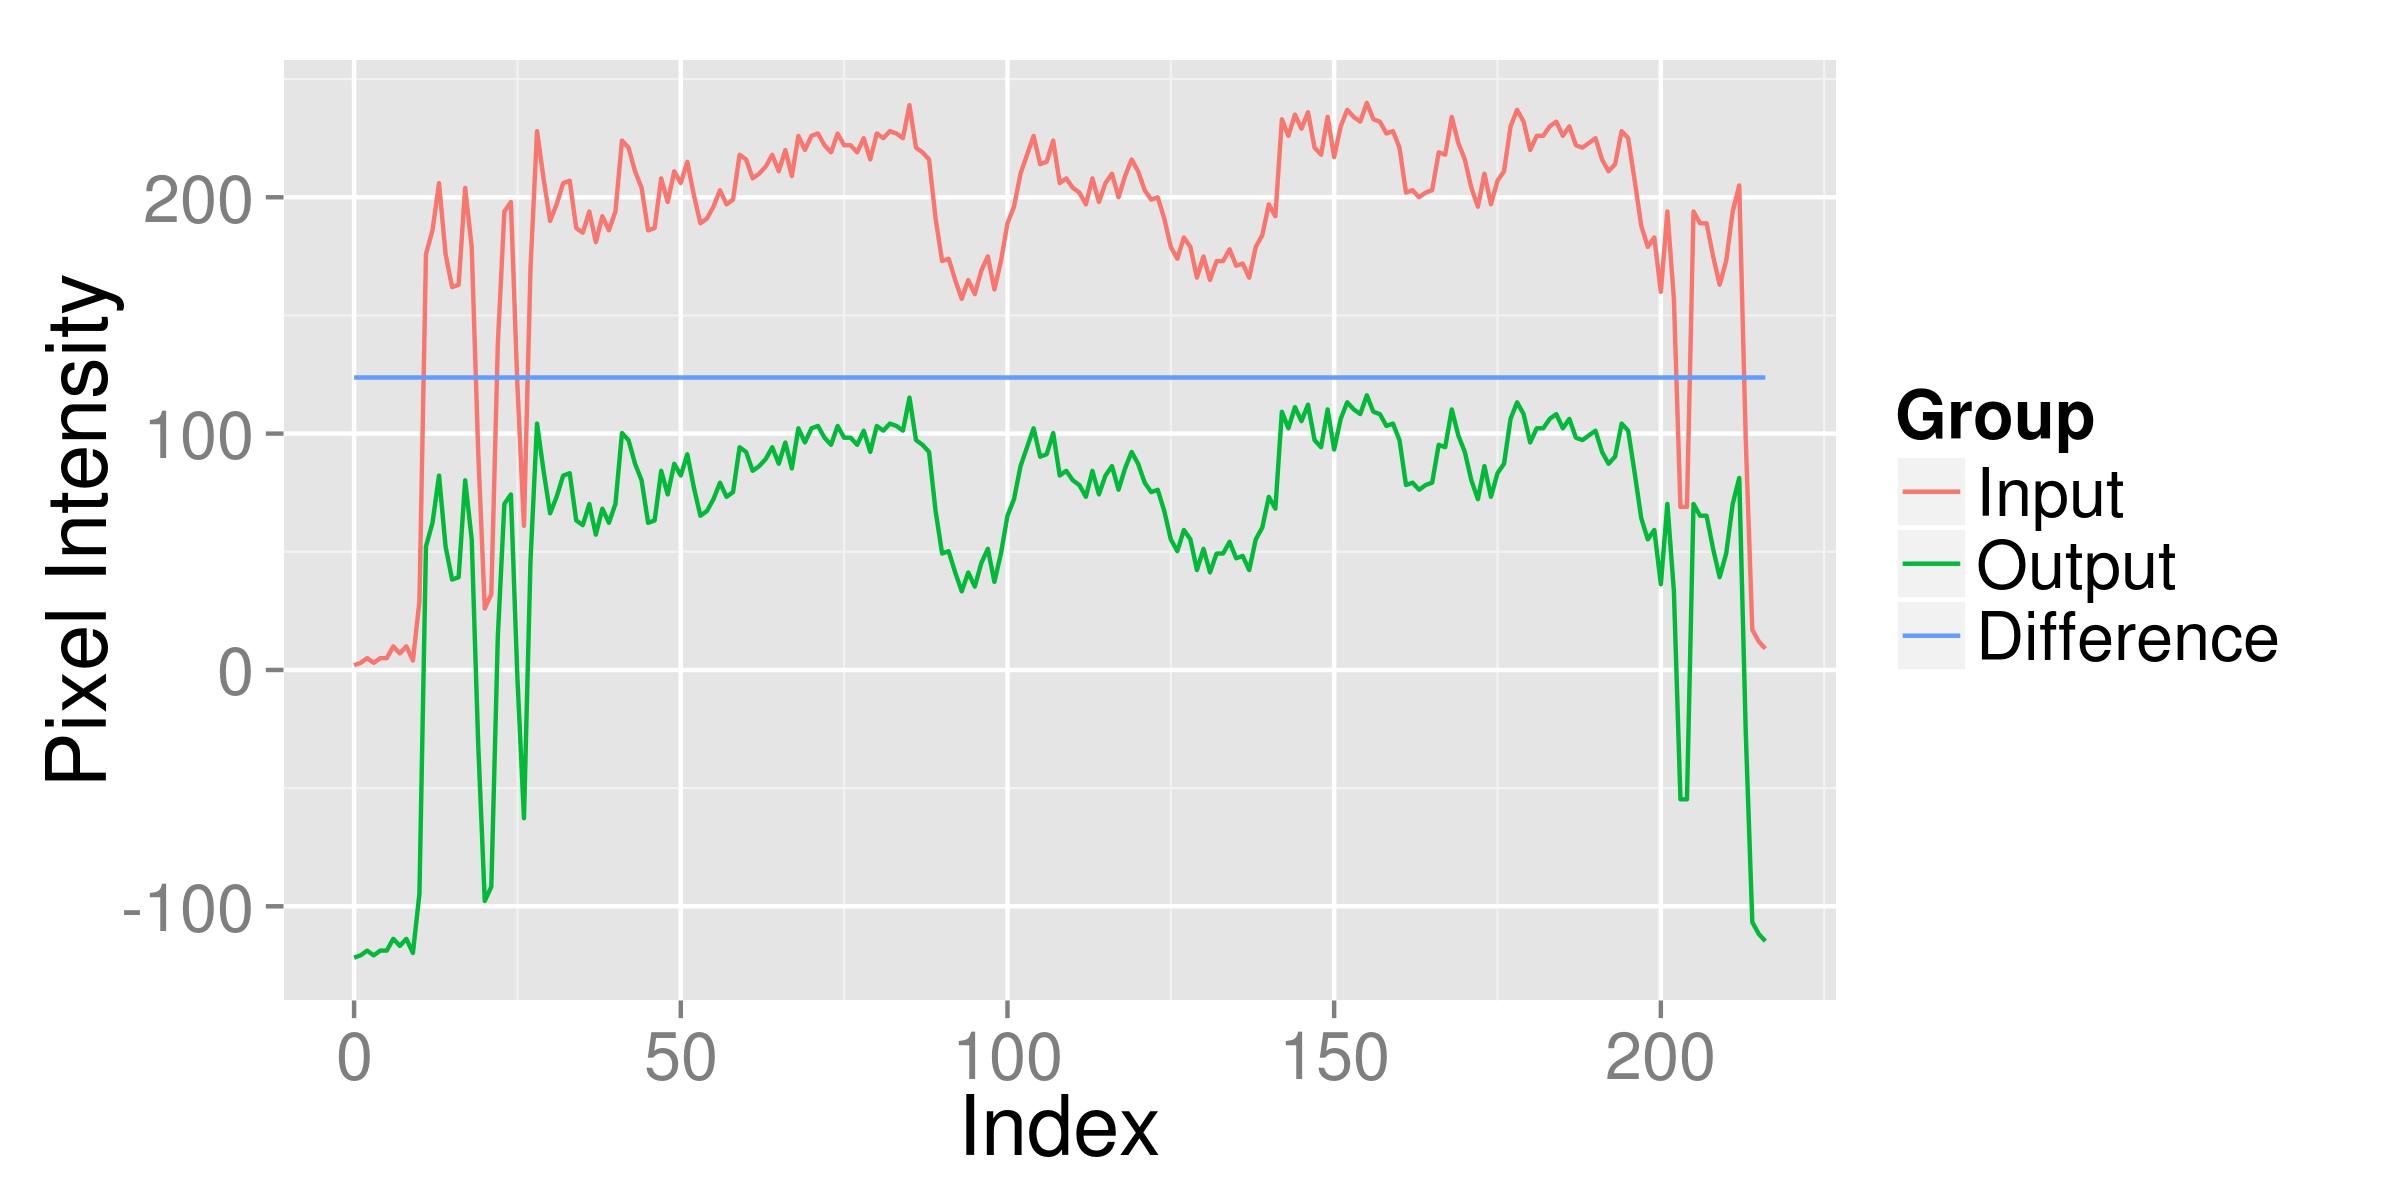
\includegraphics[width=0.8\textwidth]{images/appendix/additive_constant.png}
\itkcaption[Additive]{Plot of grayscale intensities along the vertical centerline of the input and output images.  Note that the two curves differ by an additive constant.}
\label{fig:Additive}
\end{figure}

%%%%%%%%%%%%%%%%%%%%%%%%%%%%%%%%%%%%%%%%%
%
%  Insert the bibliography using BibTeX
%
%%%%%%%%%%%%%%%%%%%%%%%%%%%%%%%%%%%%%%%%%

\bibliographystyle{plain}
\bibliography{InsightJournal}


\end{document}

